\documentclass[12pt,letterpaper]{article}
\usepackage[utf8]{inputenc}
\usepackage{fontenc}

\renewcommand{\familydefault}{\sfdefault}

\usepackage[spanish]{babel} %Reglas españolas para división de sílabas, traducción de comandos, etc...
\usepackage{amsmath}
\usepackage{amsfonts}
\usepackage{amssymb}
\usepackage{makeidx}
\usepackage{graphicx,graphics} %para imagenes
\usepackage{setspace} %Este paquete añade las funciones "\doublespacing" interlineado doble, "\onehalfspacing" interlineado de 1.5 y "\singlespacing" interlineado simple 
%\usepackage[none]{hyphenat} % Evita separar las palabras en todo el documento
%\hyphenation{palabra1, palabra2} para evitar que se separen las palabras que se encuentra entre corchetes


\usepackage{tabularx}

\usepackage[left=3cm,right=3cm,top=0.5cm,bottom=3cm,includehead]{geometry} % margen de 3cm a cada lado menos arriba
\usepackage{fancyhdr} %encabezados
\setlength{\headheight}{2cm}
%\setlength{\headheight}{\textwidth}
\pagestyle{fancy} %agrega los encabezados en todas las paginas
\fancyhf{} %borra encabezado y pie de pagina existentes
%\fancyhead[L] {\includegraphics[width = 14cm]{g3495.png}}
\renewcommand{\headrulewidth}{0pt} % elimina la raya que separa el encabezado%  %%%%    %%%\fancyhead[L] {\includegraphics[height = \headheight ]{logo.jpg}}
\parskip=2mm

\usepackage{endnotes}
\let\footnote=\endnote
\renewcommand{\notesname}{}

%\setlength{\extrarowheight}{4pt}

%-------- configuracion de la Caja -----------------
\usepackage{fancybox}
%\setlength{\fboxsep}{10pt}
\setlength{\shadowsize}{1pt} %grosor de la sombra
%----------------------------------------------------

%\graphicspath{/home/abr1l/carpeta personal/ubuntu/Manual IRC/imagenes}

\title{Manual de Instalaci\'on del IRC}
\author{Milagros Nazaret Lopez Colmenarez}
\date{}
\begin{document}

\begin{center}
{\bf \large Manual de Instalaci\'on del IRC}\footnote{Hecho en {\large\LaTeX} por por Milagros López y David Hernández para la comunidad Ubuntu-ve.}
\end{center}

En este peque\~no manual se explicar\'a c\'omo instalar \textit {HexChat}, uno de los tantos cliente que se utiliza para conectarse a los canales IRC, se ha seleccionado por ser uno de los más sencillos de manejar.

El IRC y sus canales son muy usados para dar soporte en la red, es simple, de texto plano, no tiene gif y/o emoticones que pueden distraer, aunque fue creado en 1988 se sigue utilizando para consultas y por qué no, también para socializar.

\textbf {IRC (Internet Relay Chat)} es un protocolo de comunicaci\'on en tiempo real basado en texto, que permite debates entre dos o m\'as personas. La principal diferencia de la mensajer\'ia instant\'anea es que los usuarios no necesitan establecer comunicaci\'on de antemano, de tal forma que todos los usuarios que se encuentran en un canal pueden comunicarse entre s\'i, aunque no hayan tenido ning\'un contacto anterior. Las conversaciones se desarrollan en los llamados canales de IRC, designados por nombres que habitualmente comienzan con el car\'acter ``\#". Es un sistema de charlas ampliamente utilizado por personas de todo el mundo.

Los usuarios del IRC utilizan una aplicaci\'on cliente para conectarse con un servidor, en el que funciona una aplicaci\'on IRCd (IRC daemon o servidor de IRC) que gestiona los canales y las conversaciones murales.


Ahora, procedemos a instalar HexChat,  HexChat es un \textit{fork} del cliente XChat, nos servir\'a para poder conectarnos al canal \texttt{\#ubuntu-ve}. 

\begin{enumerate}
\item Lo primero que debemos hacer es abrir una terminal, en escritorios basados en Gnome se puede acceder a trav\'es  de la combinaci\'on de teclas \verb!Ctrl + Alt + t! (al mismo tiempo). 

Una vez dentro del terminal procedemos a actualizar la lista de paquetes que tenemos disponibles, esto lo haremos escribiendo lo siguiente:

\begin{verbatim}
sudo apt-get update
\end{verbatim}

\item Actualizados los paquetes procedemos a descargar HexChat escribimos el siguiente comando en el terminal:

\begin{verbatim}
sudo apt-get install hexchat
\end{verbatim}

\item Ya lo tenemos instalado, ahora abrimos el programa y nos mostrará lo siguiente:

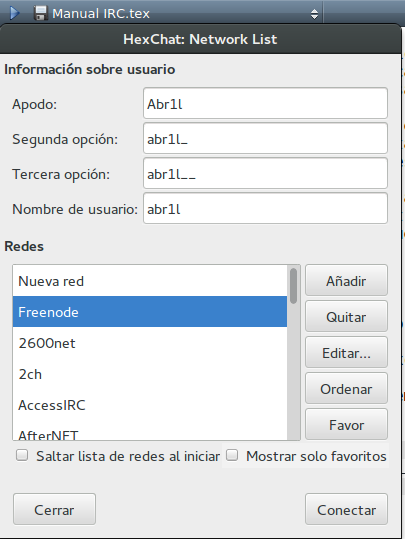
\includegraphics[width = 7cm]{imagenes/imagen1.png}

Como se puede apreciar nos solicita información con respecto a nuestro apodo (o \textit{nickname} en inglés), y dos alternativas más, además de nuestro nombre real.

En nuestro caso nos interesa entrar al servidor \textit{freenode}, el cual configuraremos para que el programa se conecte a él automáticamente al iniciar.

\begin{enumerate}
\item Comenzamos haciendo click en \textbf{Editar}. Luego click en la pestaña \textbf{Autoentrar a los canales}. Aquí iremos agregando los canales que deseamos mantener, recordando que los canales comienzan con el carácter ``\#", escribiremos \texttt{\#ubuntu-ve} al seleccionar la opci\'on \textbf{A\~nadir}.

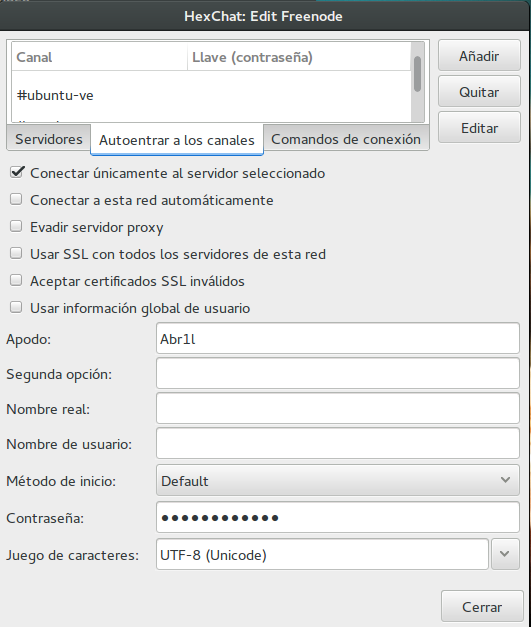
\includegraphics[width = 7cm]{imagenes/imagen2.png}

\item Cerramos y nos conectamos, ahora, cada vez que nos conectemos al servidor \texttt{freenode}, \'este lo hará autom\'aticamente al canal de \texttt{\#ubuntu-ve}, a medida que usemos la herramienta, sin lugar a dudas, iremos agregando más canales al cliente IRC.
\end{enumerate}

\item Luego de habernos conectado veremos el canal \texttt{\#ubuntu-ve} en la barra lateral izquierda, lo siguiente ser\'a escribir, comentar, preguntar y/o aportar en la caja de texto que se encuentra en la parte inferior de HexChat.

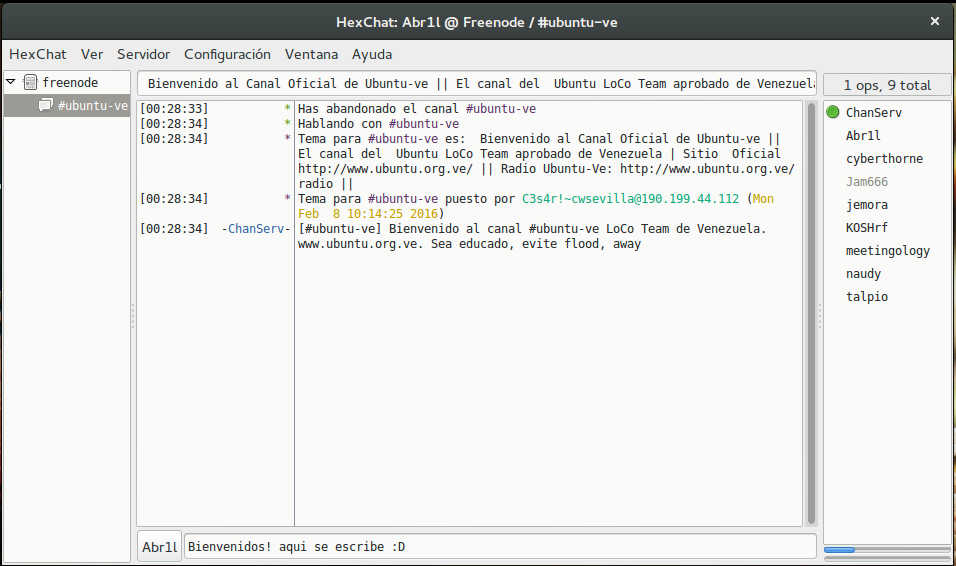
\includegraphics[width = 14cm]{imagenes/imagen4.png}

\end{enumerate}

\begin{center} % Centra el Texto
{\bf \large Comandos usados en el IRC} % Negrilla
\end{center}

Ahora que ya tenemos instalado nuestro cliente aprendamos un poco sobre el manejo de los comandos en el IRC.

La sintaxis de todos los comandos en los canales, comienza siempre con el carácter ``{\bfseries\itshape /}"

Algunos comandos son:

\begin{tabularx}{15cm}{||l|X|l||}
\hline\hline
\textbf{Comando} & \textbf{Descripci\'on}  & \textbf{Uso} \\
\hline \hline
{\bfseries\itshape /}whois & Ver informaci\'on de un usuario, si está conectado y/o en que canales se encuentra & \texttt{/whois Abr1l} \\
\hline
{\bfseries\itshape /}who & Ver usuarios en un canal aunque no se esté adentro de él & \texttt{/who \#ubuntu-ve} \\
\hline 
{\bfseries\itshape /}join & Entrar o crear un canal & \texttt{/join \#ubuntu-es} \\
\hline
{\bfseries\itshape /}nick & Cambiar el nick (apodo) actual por otro & \texttt{/nick Abril} \\
\hline
{\bfseries\itshape /}part & Salir de un canal con un comando & \texttt{/part} \\
\hline 
{\bfseries\itshape /}me & Enviar un mensaje como acci\'on, por ejemplo: Abr1l est\'a feliz & \texttt{/me est\'a feliz} \\
\hline
{\bfseries\itshape /}ignore & Ignorar un nick & \texttt{/ignore Abr1l} \\
\hline\hline
\end{tabularx} 

\begin{center} % Centra el Texto
{\bf \large Registrando el apodo en IRC y enmascarando la IP} % Negrilla
\end{center}

Ya tenemos todo lo necesario para usar esta herramienta, ahora aprenderemos a registrar nuestro apodo y luego a enmascarar nuestra ip para evitar que esta se muestre.

?`Para qu\'e registrar nuestro apodo? Pues as\'i s\'olo nosotros lo podr\'iamos usar, y siempre que aparezca ese apodo en cualquier canal sepan que somos nosotros, los pasos son: 

\begin{enumerate}

\item Escoger un apodo (\textit{nick}) que no se encuentre ya registrado.

\item En \textsl{freenode}, escribiremos:\\
\verb!/msg NickServ REGISTER nuestra-contraseña nuestro-correo!

\item Si todo sale bien, recibiremos un correo con un comando y un c\'odigo de confirmaci\'on. El comando es:\\
\verb!/msg NickServ VERIFY REGISTER nuestro-nick código-recibido!

\item Ahora, cada vez que nos conectemos debemos usar el siguiente comando para autenticarnos: \\
\verb!/msg NickServ identify nuestra-contraseña!
    
\item Para solicitar el enmascaramiento (\textit{cloak}) de nuestra ip entraremos al canal \textsl{freenode}, \texttt{/join \#freenode} y solicitaremos hablar con un \textit{staff} (en inglés). Una vez en el canal escribimos \texttt{/stats p} para mostrar los staff activos y luego escribimos: \textit{ Hi, can you help me? Please, I would like to get my nick cloaked.}  y nos contestar\'an, en ingl\'es, inform\'andonos que tenemos cloak (enmascaramiento de la ip).

\end{enumerate}

%\begin{itemize}
%\item[\bf /whois ] Ver información de un usuario, si esta conectado y/o en que canales se encuentra p.e. /whois abr1l

%\item[\bf /join] Entrar o crear un canal p.e. /join \#ubuntu-ve


%\end{itemize}
\noindent\rule{\textwidth}{1pt}

\begin{center}

\includegraphics[scale=.75]{imagenes/cc-by.png}\\
Este obra está bajo una licencia de Creative Commons Reconocimiento 4.0 Internacional.
\end{center}


\theendnotes
\end{document}